\documentclass[border=6pt]{standalone}
\usepackage[T1]{fontenc}
\usepackage[utf8]{inputenc}
\usepackage[scaled=0.98]{helvet}
\renewcommand{\familydefault}{\sfdefault}
\usepackage{amsmath}
\usepackage{graphicx}
\graphicspath{{../../../../../../exercises_lecturenotes/lecture_notes/kurs100_lektionsnoter/}}
\usepackage{tikz}
\usepackage{pgfplots}
\pgfplotsset{compat=1.18}
\usetikzlibrary{arrows.meta, decorations.pathreplacing, calc, positioning, fit, backgrounds, shapes.geometric}
\usepgfplotslibrary{groupplots,fillbetween}
\definecolor{scanpink}{HTML}{E5006D}
\definecolor{scanteal}{HTML}{00A6A6}
\definecolor{scannavy}{HTML}{243746}
\definecolor{scanlightgray}{HTML}{F1F2F3}
\begin{document}
  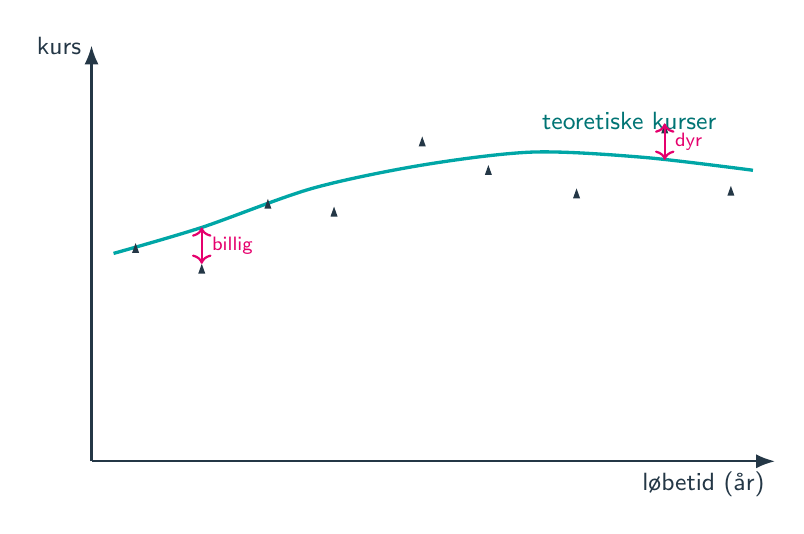
\begin{tikzpicture}[x=0.28cm,y=0.33cm,font=\small]
    \draw[-{Latex[length=2.4mm]},thick,scannavy] (0,0) -- (31,0) node[below left] {løbetid (år)};
    \draw[-{Latex[length=2.4mm]},thick,scannavy] (0,0) -- (0,16) node[left] {kurs};
    \draw[very thick,scanteal] plot[smooth] coordinates {(1,8)(5,9)(10,10.5)(15,11.4)(20,11.9)(25,11.7)(30,11.2)};
    \node[scanteal!70!black,anchor=west] at (20,13.1) {teoretiske kurser};
    \foreach \x/\y in {2/8.4,5/7.6,8/10.1,11/9.8,15/12.5,18/11.4,22/10.5,26/13.0,29/10.6}
      \fill[scannavy] (\x,\y) -- ++(-0.16,-0.38) -- ++(0.32,0) -- cycle;
    \draw[<->,thick,scanpink] (5,7.6) -- (5,9) node[midway,right,font=\scriptsize] {billig};
    \draw[<->,thick,scanpink] (26,11.6) -- (26,13.0) node[midway,right,font=\scriptsize] {dyr};
  \end{tikzpicture}
\end{document}
